\section{Interactions}\label{interactions}

Through the iterations described in the previous chapter, we arrived at
Foldlings' tool-based system for card design.

\subsection{Tool Interactions}\label{tool-interactions}

Some interactions are common to all features. To add a feature . Tool
modes

\begin{quote}
\begin{quote}
TODO: add tap options, how to draw, and a description of the tool-based
interface in general
\end{quote}
\end{quote}

\subsubsection{Box Fold}\label{box-fold}

To draw a

\subsubsection{FreeForm}\label{freeform}

\subsubsection{Polygon}\label{polygon}

\subsubsection{V-Fold}\label{v-fold}

The only action that can be performed on a v-fold feature is deletion.

\subsection{Tutorial}\label{tutorial}

We eschewed detailed drawing instructions or a separate tutorial mode,
in favor of short video tutorials that appear the first time each tool
is used. These tutorials can also be accessed by tapping the feature
icons on the about page.

\begin{figure}[htbp]
\centering
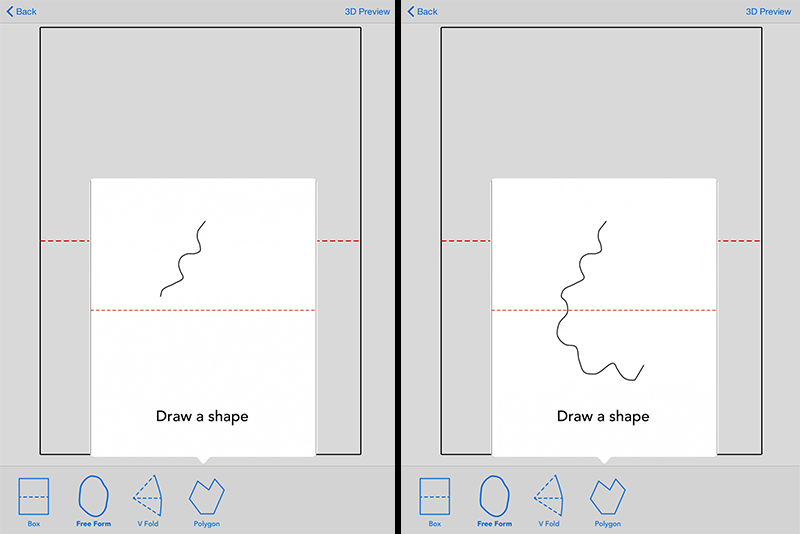
\includegraphics{figures/32_UI_Tool_Interactions/tutorial_step_one_two.png}
\caption{Free-form shape tutorial video.}
\end{figure}

We also show helpful tips between screens --- for example, when moving
to 3D preview and restoring from a saved sketch.

\subsection{Warnings and Errors}\label{warnings-and-errors}

We display warnings and errors as bright-red banners at the top of the
sketch view when. These warnings are displayed in response to failing
the validity checks performed when adding a feature to the sketch.

\begin{figure}[htbp]
\centering
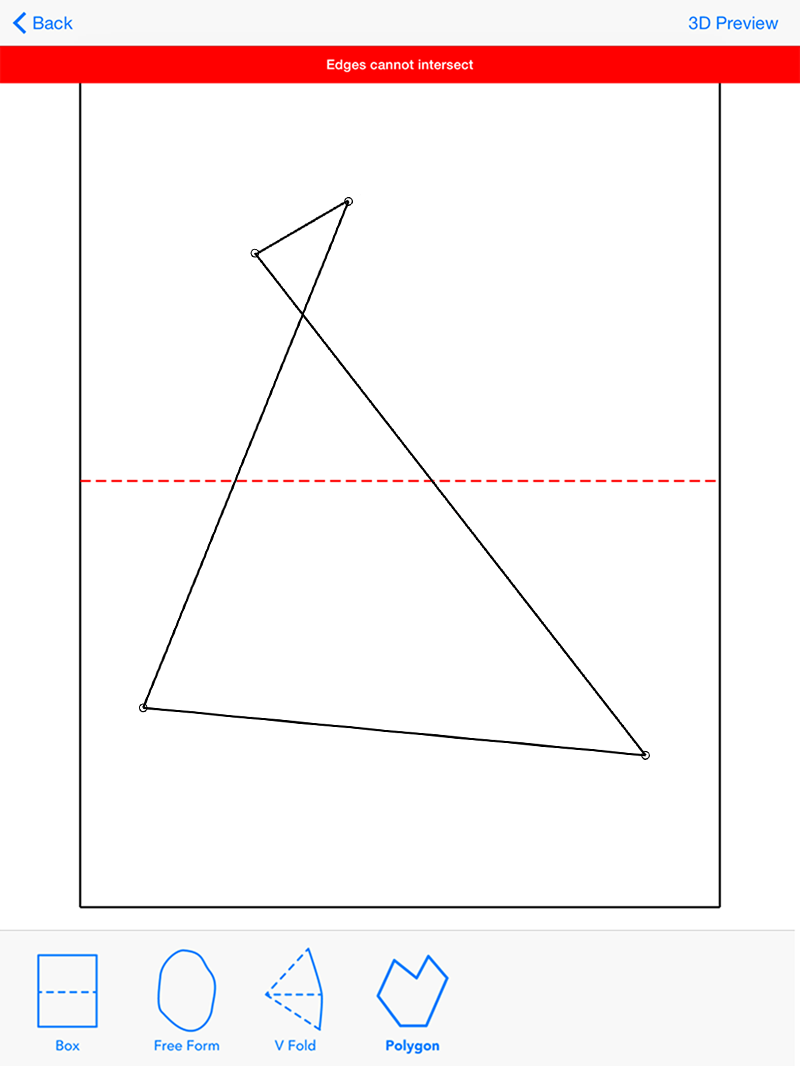
\includegraphics{figures/32_UI_Tool_Interactions/error_message.png}
\caption{An error message shown when rejecting a polygon with
intersecting edges.}
\end{figure}

The goal of these warnings is to give users descriptive feedback when
errors occur, and to give them an intuitive sense of which actions
create invalid features.

\subsection{Send to Laser Cutter}\label{send-to-laser-cutter}

In the three-dimensional preview, users can tap the ``send to laser
cutter'' option. This feature sends the user an email with an attached
SVG file. This file can be fed to a laser cutter or paper cutting
machine, or can be opened in a vector graphics program to make further
changes.

\subsection{Print}\label{print}

\begin{figure}[htbp]
\centering
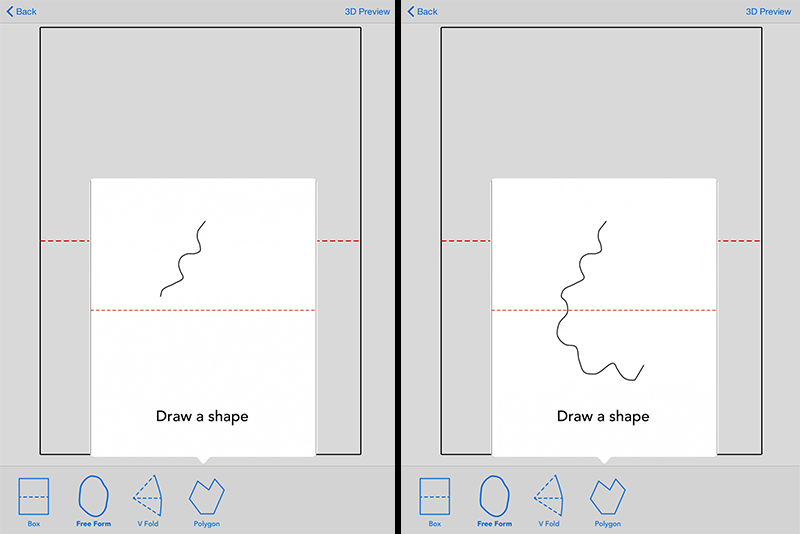
\includegraphics{figures/32_UI_Tool_Interactions/tutorial_step_one_two.png}
\caption{Options for sharing a fold pattern from the 3D preview.}
\end{figure}
